\chapter{Method}
This chapter lists all the used data sets and explains the procedure.

\section{Public plant disease datasets}
\label{section:plant_datasets}

There are several datasets on plant diseases publicly available, but only a few meet the requirements such as sufficient size and appropriate image resolution. The following Table~\ref{tab:suitable_plant_datasets} lists the suitable plant disease datasets used in this work. The complete list regarded plant datasets including links is in the Appendix~\ref{appendix:datasets_tables}.

\begin{table}[H]
\centering
\caption{Large plant disease datasets\label{tab:suitable_plant_datasets}}
\begin{tabularx}{\textwidth}{|
 >{\hsize=.72\hsize}X |
 >{\hsize=.14\hsize\raggedleft}X |
 >{\hsize=.14\hsize\raggedleft}X |
}
\hline
\textbf{Name} & \textbf{\#Images} & \textbf{\#Classes} \tabularnewline \hline
\gls{pvd} \autocite{hughes2016} & 54'303 & 38 \tabularnewline \hline
Cassava Leaf Disease Classification \autocite{mwebaze2020} & 21'398 & 5 \tabularnewline \hline
PlantDataset \autocite{pal2022} & 5'106 & 20 \tabularnewline \hline
PlantDoc \autocite{singh2020} & 2'598 & 28 \tabularnewline \hline
\gls{darma} \autocite{keaton2021} & 231'414  & 1'000 \tabularnewline \hline
\gls{pddd} \autocite{dong2023} & 421'133  & 120 \tabularnewline \hline
\end{tabularx}
\end{table}

All datasets were checked for obvious duplicates and cleaned up if necessary. Some of the datasets have additional label errors and near duplicates with different magnifications or similar small changes \autocite{groeger2023}. These changes make it harder to detect such cases. For the sake of simplicity the duplicate check in this work only covers images with the exact same image hash or the same file name combined with manual verification. The complete list of cleaning steps is in the Appendix~\ref{appendix:data_quality_assessment}.

\subsection{PlantVillage Dataset (PVD)}
The \gls{pvd} contain 54'303 images and is therefore one of the larger plant disease data sets available. Accordingly it is often used in other work \autocite{hughes2016}, but there is no official test split provided to compare the results of already existing models. Some achieved an accuracy around 90\% with the ResNet50 architecture \autocite{gole2023}.

All images in the dataset have a lab-controlled background as shown in Figure~\ref{fig:example_images_of_plantvillage}.
\begin{figure}[H]
    \begin{center}
    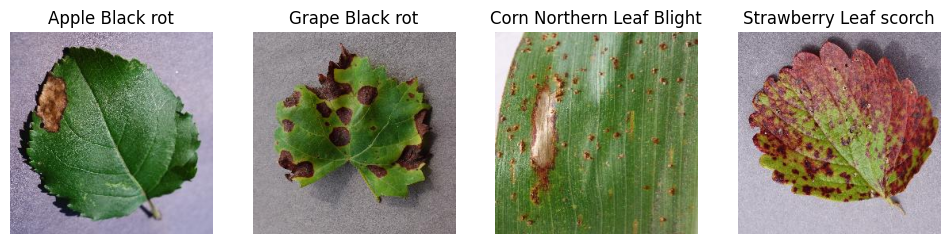
\includegraphics[width=15cm]{../images/example_images_of_plantvillage.png}
    \caption{Example images of the \gls{pvd}}\label{fig:example_images_of_plantvillage}
    \end{center}
\end{figure}

This dataset does not provide a split for a test test. Therefore, the splitting was carried out by myself using 80\% of the data for the training set and 10\% each for the validation and test set. The stratifying ensures, that the distribution of the 38 classes is the same over all sets, which can be seen in Figure~\ref{fig:class_distribution_of_plantvillage}. 
\begin{figure}[H]
    \begin{center}
    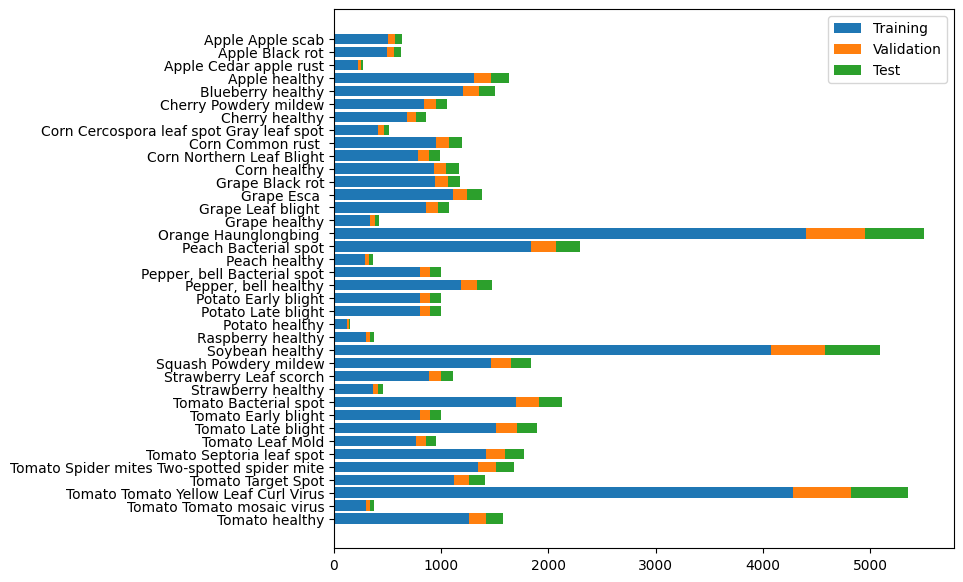
\includegraphics[width=15cm]{../images/class_distribution_of_plantvillage.png}
    \caption{Class distribution of PlantVillage}\label{fig:class_distribution_of_plantvillage}
    \end{center}
\end{figure}



% Without a given split is also not possible to have a meaningful line.


\subsection{Cassava Leaf Disease Classification}
Figure~\ref{fig:example_images_of_cassava}.

\begin{figure}[H]
    \begin{center}
    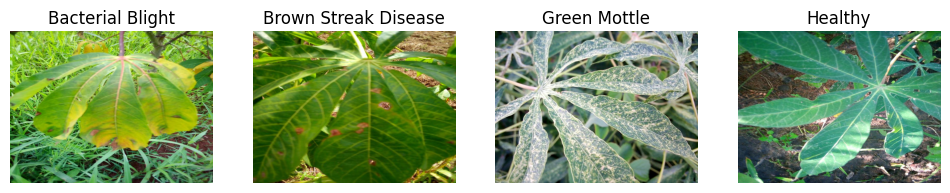
\includegraphics[width=15cm]{../images/example_images_of_cassava.png}
    \caption{Example images of Cassava}\label{fig:example_images_of_cassava}
    \end{center}
\end{figure}

Figure~\ref{fig:class_distribution_of_cassava}

\begin{figure}[H]
    \begin{center}
    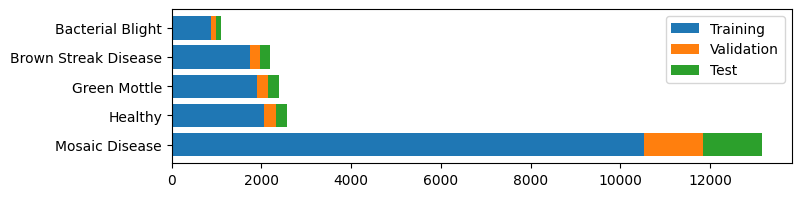
\includegraphics[width=15cm]{../images/class_distribution_of_cassava.png}
    \caption{Class distribution of Cassava}\label{fig:class_distribution_of_cassava}
    \end{center}
\end{figure}


\subsection{PlantDataset}

Figure~\ref{fig:example_images_of_plantdataset}.

\begin{figure}[H]
    \begin{center}
    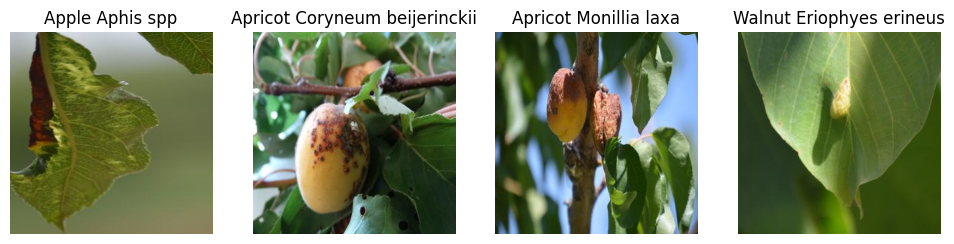
\includegraphics[width=15cm]{../images/example_images_of_plantdataset.png}
    \caption{Example images of PlantDataset}\label{fig:example_images_of_plantdataset}
    \end{center}
\end{figure}

Figure~\ref{fig:class_distribution_of_plantdataset}

\begin{figure}[H]
    \begin{center}
    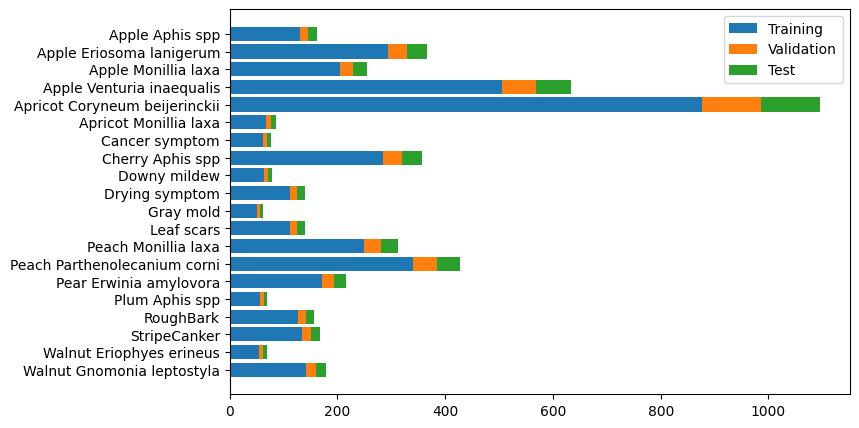
\includegraphics[width=15cm]{../images/class_distribution_of_plantdataset.png}
    \caption{Class distribution of PlantDataset}\label{fig:class_distribution_of_plantdataset}
    \end{center}
\end{figure}

\subsection{PlantDoc}
Figure~\ref{fig:example_images_of_plantdoc}.

\begin{figure}[H]
    \begin{center}
    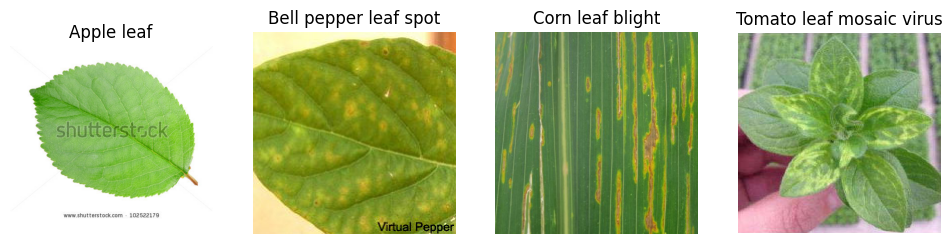
\includegraphics[width=15cm]{../images/example_images_of_plantdoc.png}
    \caption{Example images of PlantDoc}\label{fig:example_images_of_plantdoc}
    \end{center}
\end{figure}

Figure~\ref{fig:class_distribution_of_plantdoc}

\begin{figure}[H]
    \begin{center}
    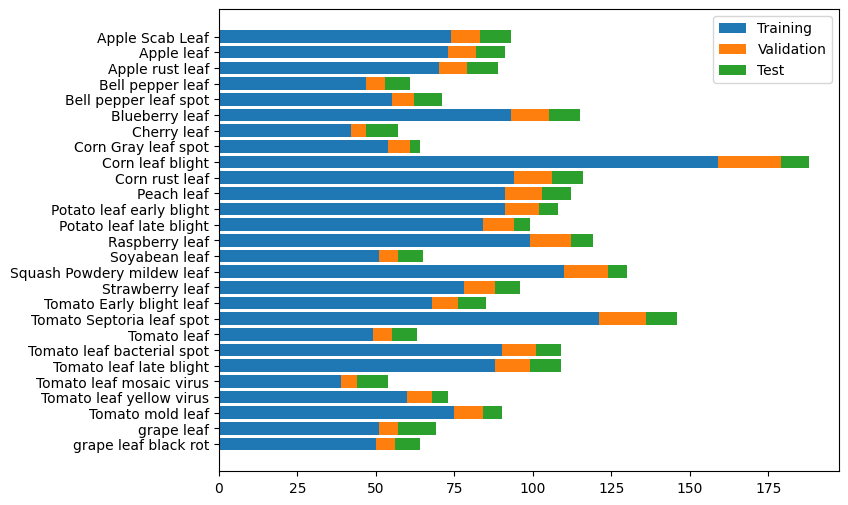
\includegraphics[width=15cm]{../images/class_distribution_of_plantdoc.png}
    \caption{Class distribution of PlantDoc}\label{fig:class_distribution_of_plantdoc}
    \end{center}
\end{figure}

\subsection{DARMA}

Figure~\ref{fig:example_images_of_darma}.

\begin{figure}[H]
    \begin{center}
    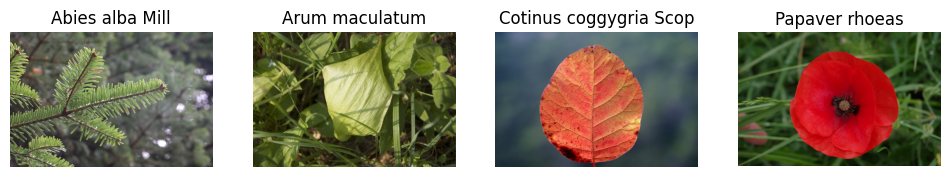
\includegraphics[width=15cm]{../images/example_images_of_darma.png}
    \caption{Example images of \gls{darma}}\label{fig:example_images_of_darma}
    \end{center}
\end{figure}

\subsection{Plant Disease Diagnosis Dataset (PDDD)}

Figure~\ref{fig:example_images_of_pddd}.

\begin{figure}[H]
    \begin{center}
    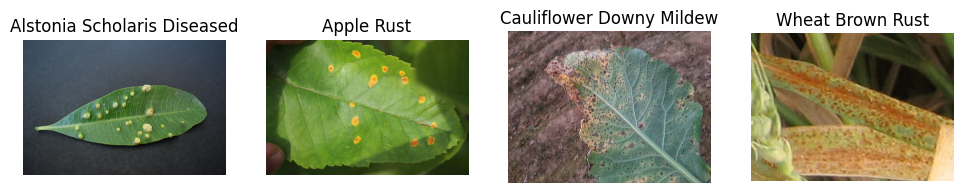
\includegraphics[width=15cm]{../images/example_images_of_pddd.png}
    \caption{Example images of \gls{pddd}}\label{fig:example_images_of_pddd}
    \end{center}
\end{figure}


\section{Public dermatology datasets}
\label{section:derma_datasets}

%TODO: replace citations
\begin{table}[H]
\centering
\caption{Dermatology datasets\label{tab:suitable_derma_datasets}}
\begin{tabularx}{\textwidth}{|
    >{\hsize=.72\hsize}X |
    >{\hsize=.14\hsize\raggedleft}X |
    >{\hsize=.14\hsize\raggedleft}X |
}
\hline
\textbf{Name} & \textbf{\#Images} & \textbf{\#Classes} \tabularnewline \hline
PAD-UFES-20 \autocite{hslu} & ? & ? \tabularnewline \hline
\gls{ddi} \autocite{hslu} & ? & ? \tabularnewline \hline
HAM10000 \autocite{hslu} & ? & ? \tabularnewline \hline
Fitzpatrick17k \autocite{hslu} & ? & ? \tabularnewline \hline
\end{tabularx}
\end{table}

\subsection{PAD-UFES-20}
Figure~\ref{fig:example_images_of_pad-ufes-20}.

\begin{figure}[H]
    \begin{center}
    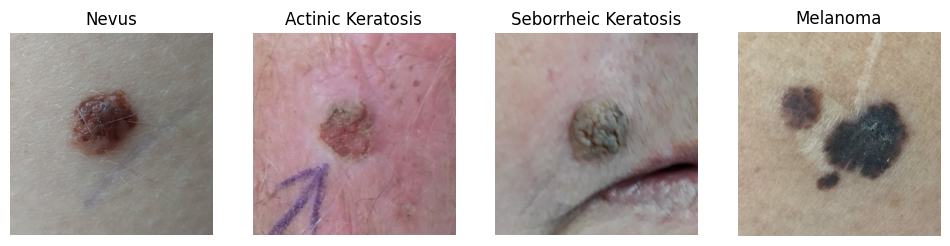
\includegraphics[width=15cm]{../images/example_images_of_pad-ufes-20.png}
    \caption{Example images of PAD-UFES-20}\label{fig:example_images_of_pad-ufes-20}
    \end{center}
\end{figure}

Figure~\ref{fig:class_distribution_of_pad-ufes-20}

\begin{figure}[H]
    \begin{center}
    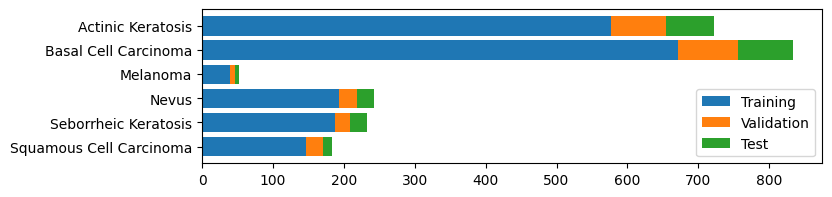
\includegraphics[width=15cm]{../images/class_distribution_of_pad-ufes-20.png}
    \caption{Class distribution of PAD-UFES-20}\label{fig:class_distribution_of_pad-ufes-20}
    \end{center}
\end{figure}
\subsection{Diverse Dermatology Images (DDI)}
Figure~\ref{fig:example_images_of_ddi}.

\begin{figure}[H]
    \begin{center}
    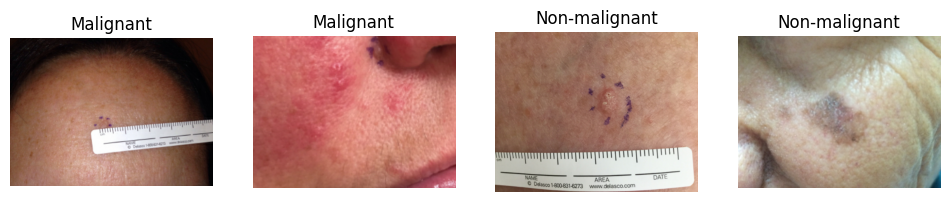
\includegraphics[width=15cm]{../images/example_images_of_ddi.png}
    \caption{Example images of \gls{ddi}}\label{fig:example_images_of_ddi}
    \end{center}
\end{figure}

Figure~\ref{fig:class_distribution_of_ddi}

\begin{figure}[H]
    \begin{center}
    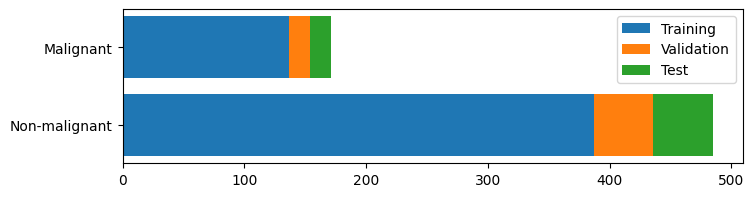
\includegraphics[width=15cm]{../images/class_distribution_of_ddi.png}
    \caption{Class distribution of \gls{ddi}}\label{fig:class_distribution_of_ddi}
    \end{center}
\end{figure}
\subsection{HAM10000}
Figure~\ref{fig:example_images_of_ham10000}.

\begin{figure}[H]
    \begin{center}
    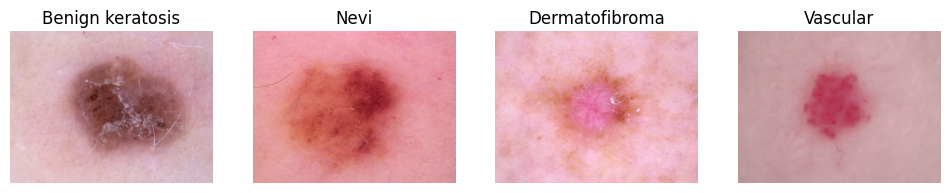
\includegraphics[width=15cm]{../images/example_images_of_ham10000.png}
    \caption{Example images of HAM10000}\label{fig:example_images_of_ham10000}
    \end{center}
\end{figure}

Figure~\ref{fig:class_distribution_of_ham10000}

\begin{figure}[H]
    \begin{center}
    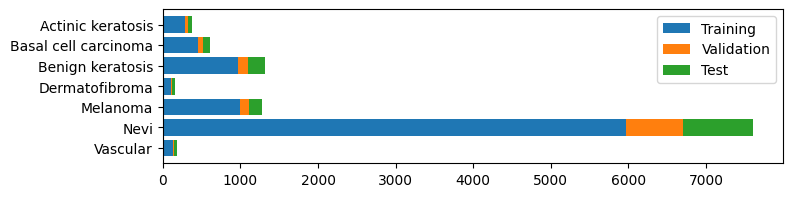
\includegraphics[width=15cm]{../images/class_distribution_of_ham10000.png}
    \caption{Class distribution of HAM10000}\label{fig:class_distribution_of_ham10000}
    \end{center}
\end{figure}
\subsection{Fitzpatrick17k}
Figure~\ref{fig:example_images_of_fitzpatrick17k}.

\begin{figure}[H]
    \begin{center}
    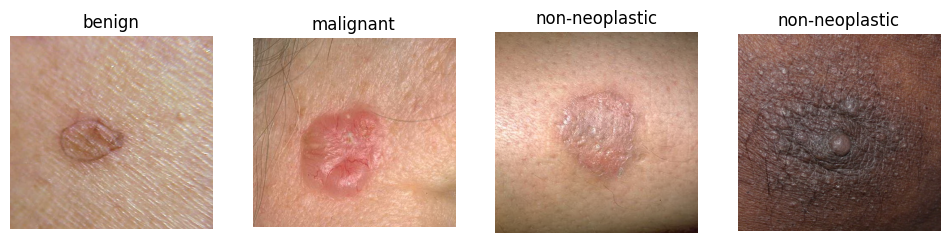
\includegraphics[width=15cm]{../images/example_images_of_fitzpatrick17k.png}
    \caption{Example images of Fitzpatrick17k}\label{fig:example_images_of_fitzpatrick17k}
    \end{center}
\end{figure}

Figure~\ref{fig:class_distribution_of_fitzpatrick17k}

\begin{figure}[H]
    \begin{center}
    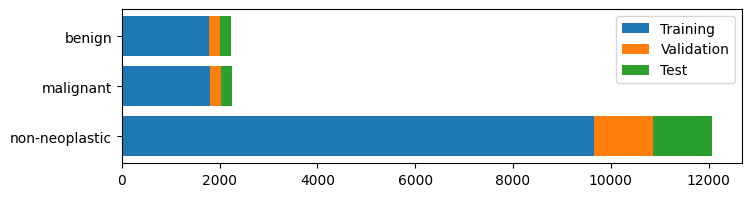
\includegraphics[width=15cm]{../images/class_distribution_of_fitzpatrick17k.png}
    \caption{Class distribution of Fitzpatrick17k}\label{fig:class_distribution_of_fitzpatrick17k}
    \end{center}
\end{figure}
